\documentclass[main]{subfiles}

\begin{document}
	\subsection{Подгруппа, составленная из степеней данного элемента. Связь порядка группы и порядка элемента. Теорема Эйлера}

	\begin{consequence}
	    G --- кон. группа,\q $a \in G$, $\ord a = m$, $H=\{a^n:n \in \Z\}$, \ тогда $|H|=m$
    \end{consequence}

	\begin{proof}
	    $\{a^0=e,a^1,...,a^{m-1}\}$ --- подмножество H\\
	    Докажем, что все остальные элементы тоже здесь есть:
	    \[n \in \Z \RA n=m q+r,\q 0 \leq r \leqslantr \leqslant m-1\]
	    \[a^n=a^{m q+r}=(a^m)^q a^r=a^r\]
	    \[a^k=a^l$,\q $0 \leqslant k \leqslant l \leqslant m-1,\q \text{умножим на } a^{-k}\]
	    \[e=a^{l-k},$ $\q 0 \leqslant l-k \leqslant m-1\q \text{m --- наименьшее $\N$ такое что $a^m=e$}\]
	    \[l-k=0 \RA l=k\]
	    Доказали, что $|H|=m$
	    \[\Ra |G| \devides m=\ord a\]
		Т.о. в группе порядок эл-та --- делитель порядка группы
	\end{proof}

	\begin{reminder}
		$n \in \N,\q \varphi(n) = \abs{\Br{\Z /_n \Z}^*} = \abs{\{1 \leq m < n: (m,\ n) = 1\}}$
	\end{reminder}

    \begin{reminder}[теорема Эйлера]
        $n,a \in \N$,\q $(a,n) = 1$,\q тогда $a^{\varphi(n)} \equiv 1 \ (\text{mod } n)$
    \end{reminder}

	\begin{proof}
        Рассмотрим $G=\Z _{n}^*$ (мультипликативная группа) $\q |G|=\varphi(n) \q$ %(группа по умножению)
	    \[\ol{a} \in G$, $\ord \ol{a}=k\]
	    \[\varphi(n) \devides k \Ra \varphi(n) = kl\]
	    %\[\ol{a}=\ol{1}\]
        \[\overline{a} \in \Z_n^* \q (a, n) = 1\]
	    \[\ol{a}^{\varphi(n)}=\ol{1}\]
	\end{proof}

	\begin{consequence}[малая т. Ферма]
		$p$ --- простое, $a^{p - 1} = 1\ (mod\ p)$
	\end{consequence}

	\subsection{Циклические группы. Примеры. Классификация циклических групп. Группы простого порядка. Прямое произведение групп остатков}
	\begin{definition}
	    G --- циклическая группа, если:
		\[\e g \in G: \forall g' \in G: \e k \in \Z: g'=g^k\]
	    Такой g называется образующим
	\end{definition}

	\begin{example}
		\begin{enumerate}
			\item $\Z$ (образующий --- единица и минус единица)
			\item Любая циклическая группа --- коммутативна
			\[g'' g' \os{?}{=} g' g'' = g^k g^l = g^l g^k\]
			\item Любая некомут. группа не явл. цикл.
		\end{enumerate}
	\end{example}

	\begin{Example}
		\[\Z /_2 \Z \times \Z /_2 \Z = \{(\ol{0},\ol{0}),(\ol{0},\ol{1}),(\ol{1},\ol{0}),(\ol{1},\ol{1})\}\]
		Никакой эл-т не явл. образующим.
	\end{Example}

	\begin{utv}
	    Конечная группа порядка n является циклической тогда и только тогда, когда она содержит элемент порядка n
		\[(|G|=n, \text{ G --- циклическая }\lra\ \e g \in G: \ord g = n)\]
	\end{utv}

	\begin{example}
		Рассмотрим $\Z /_2 \Z \times \Z /_3 \Z$ --- циклическая
		\[((\ol{1},\ol{1}), (\ol{0}, \ol{2}), (\ol{1}, \ol{0}), (\ol{0}, \ol{1}), (\ol{1},\ol{2}))\]
		Рассмотрим $\Z /_2 \Z \times \Z /_4 \Z$ --- не циклическая
	\end{example}

	\begin{theorem}
	    G --- циклическая группа
		\begin{enumerate}
			\item $|G|=n \Ra G \cong \Z / n \Z$\\
			\item $|G|=\infty \Ra G \cong \Z$
		\end{enumerate}
	\end{theorem}

	\begin{proof}
		\begin{enumerate}
			\item g --- обр. G, значит $G=\{e,g,g^2,...,g^{n-1}\}$\\
			(среди них нет одинаковых)
				\[\text{Построим изоморфизм в $\Z / n \Z$:$\q \varphi(g^k)=\ol{k}$}\]
			    \[\text{Проверим, что $\varphi(g^k g^l)= \varphi(g^k)+\varphi(g^l)=\ol{k}+\ol{l}$}\]
		        \[\text{Левая часть: $\varphi(g^{k+l})=\ol{k+l} = \ol{k}+\ol{l}$}\]
			\item $G=\{...,g^{-1},e,g,g^2,...\}$\\
				(тоже нет совпадающих элементов, иначе $g^k=g^l$, при $k>l$, тогда $g^{k-l}=e$, но тогда конечное число элементов, потому что оно зацикливается через каждые $k-l$ элементов), построим отображение в $\Z$.\\
			    $\varphi(g^n)=n$ --- очевидно, биекция.\\
				$n + k = \varphi(g^n g^k)=\varphi(g^n) + \varphi(g^k)=n+k$
		\end{enumerate}
	\end{proof}

	\begin{Utv}
		\[\Z_n \times \Z_m \simeq \Z_{mn} \text{, если } (m, n) = 1 \]
	\end{Utv}

	\begin{proof}
		Нужно построить изоморфизм $[a]_{m n} \mapsto    ([a]_n,[a]_m)$
		\[[a]_{m n} = [a']_{m n} \Ra [a]_n = [a']_n$, $[a]_m=[a']_m\]
		Теперь нужно проверить биекцию

		Сюръективность:
		\[\forall b,c \in \Z$ $\e x \in \Z: \begin{cases}[x]_n=[b]_n\\ [x]_m=[c]_m \end{cases},\text{ по КТО всё хорошо}\]
		Инъективность:
		\[\left[\begin{matrix}
			[a]_n = [b]_n\\
			[a]_m = [b]_m
		\end{matrix}\right. \RA [a]_{m n} = [b]_{m n}\]
		На языке сравнений:
		\[\begin{matrix}
			a \equiv b(n)\\
			a \equiv b(m)
		\end{matrix} \RA a \equiv b (m n)\]
		На самом деле достаточно было проверить одно
	\end{proof}

	\subsection{Изоморфизм и изоморфность групп, примеры изоморфных и неизоморфных групп. Порядок элемента и его образа при изоморфизме}

	\begin{definition}
	    $\varphi: G \ra H$ --- биекция и $\varphi(g_1g_2)=\varphi(g_1) \varphi(g_2)\q \forall g_1,g_2 \in G$,\\ тогда $\varphi$ --- изоморфизм
	\end{definition}

	\begin{examples}
	    \begin{enumerate}
	        \item $D_3 \ra S_3$
			\begin{figure}[H]
				\begin{center}
					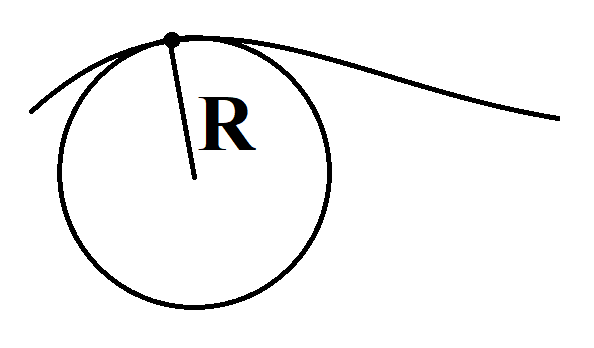
\includegraphics[width = 5cm]{2_1}
					\caption{Композиция сохраняется}
				\end{center}
			\end{figure}
	        \item $U_n=\{z\in \CC: z^n=1\} \la \Z / n \Z$\\
		        \[(\cos \frac{2\pi a}{n}+i \sin \frac{2\pi a}{n} = \varphi (\ol{a}) \leftarrow \ol{a})\]
		        \[\ol{a}=\ol{b} \ra \varphi(\ol{a})=\varphi(\ol{b})\]
		        \[\varphi(\ol{a}+\ol{b}) \overset{?}{=} \varphi(\ol{a})\varphi(\ol{b})\]
		        \[\cos \frac{2\pi(a+b)}{n}+i \sin \frac{2\pi(a+b)}{n}=(\cos\frac{2\pi a}{n} + i \sin \frac{2\pi a}{n})\]
	    \end{enumerate}
	\end{examples}

	\begin{definition}
	    Две группы называются изоморфными, если между ними существует изоморфизм
	\end{definition}

	\begin{utv}
	    Изоморфизм --- отношение эквивалентности
	\end{utv}

	\begin{proof}
	    Транзитивность: $G \overset{\varphi}{\ra} H \overset{\psi}{\ra} P$
        \[(\psi \circ \varphi)(g_1 g_2) = \psi(\varphi(g_1 g_2)) = \psi(\varphi(g_1) \varphi(g_2)) = \]
		\[= \psi(\varphi(g_1)) \psi(\varphi(g_2)) =
        (\psi \circ \varphi)(g_1) * (\psi \circ \varphi)(g_2)\]
	    Рефлексивность: тождественное отображение --- изоморфизм\\
	    Симметричность: $G \underset{\varphi}{\ra} H$, $H \underset{\varphi^{-1}}{\ra} G$
	\end{proof}

\end{document}
